\documentclass[UTF8,12pt]{ctexart}
\usepackage{geometry}
\usepackage{float}
\usepackage{amsmath}
\usepackage{graphicx}
\usepackage{listings}
\usepackage{xcolor}
\usepackage{hyperref}
\geometry{a4paper, left=2.5cm, right=2.5cm, top=2.5cm, bottom=2.5cm}
\setmonofont{Consolas}
\lstset{
	numbers=left, 
	numberstyle= \tiny, 
	keywordstyle= \color{blue!70},%设置关键字颜色
	commentstyle= \color{red!50!blue!50}, %设置注释颜色
	frame=shadowbox, % 阴影效果
	rulesepcolor= \color{ red!20!green!20!blue!20} ,
	escapeinside=``, % 英文分号中可写入中文
	aboveskip=1em,
	tabsize=2,				%此时一个tab键=2个空格
	framexleftmargin=2em,
	basicstyle=\ttfamily,
	columns=fullflexible,%可以自动换行
	linewidth=1\linewidth, %设置代码块与行同宽
	breaklines=true,%在单词边界处换行. 
	showstringspaces=false, %去掉空格时产生的下划的空格标志, 设置为true则出现
	breakatwhitespace=true,%可以在空格处换行
	escapechar=`%设置转义字符为反引号
}
\title{\textbf{Python结课作业项目报告}}
\author{Vespera Zephyr}

\date{\today}

\begin{document}
	\maketitle
	\textbf{\large 项目选题:实用工具类. }
	\tableofcontents
	\section{需求分析}
	\begin{itemize}
		\item 支持常见微积分运算
		\item 直观的公式渲染能力
		\item 友好的图形界面和帮助选项
		\item 较快的计算速度
	\end{itemize}
	
	\subsection{功能需求}
	\begin{tabular}{|l|l|}
		\hline
		\textbf{核心功能} & \textbf{实现要求} \\ 
		\hline
		符号计算 & 支持求导、积分、极限、化简等操作 \\
		输入验证 & 实时检测非法输入并提示 \\
		结果展示 & 双模式显示(文本+公式渲染) \\
		历史保存 & 计算结果可保存为结构化文本 \\
		帮助系统 & 内置符号输入规范说明 \\
		\hline
	\end{tabular}
	
	\section{设计思路}
	\subsection{架构设计}
	采用MVC模式实现:
	\begin{itemize}
		\item \textbf{Model}: Sympy符号计算引擎
		\item \textbf{View}: PyQt6图形界面
		\item \textbf{Controller}: 事件驱动逻辑控制
	\end{itemize}
	引入第三方库:
	\begin{lstlisting}[language=Python]
import sys
from datetime import datetime
from PIL import Image
from sympy import *
from sympy.parsing.sympy_parser import parse_expr
from PyQt6.QtWidgets import (
	QApplication, QMainWindow, QWidget, QVBoxLayout, QHBoxLayout,
	QLineEdit, QPushButton, QLabel, QComboBox, QGridLayout,
	QTabWidget, QFrame, QScrollArea, QMessageBox, QFileDialog,
	QDialog,        # 用于创建对话框
	QScrollArea   # 滚动区域
)
from PyQt6.QtWebEngineWidgets import QWebEngineView
from PyQt6.QtCore import  QThread, pyqtSignal, pyqtSlot
from PyQt6.QtGui import QAction
	\end{lstlisting}
	
	\subsection{关键技术}
	\begin{itemize}
		\item 多线程计算:QThread防止界面冻结
		\item 动态界面:GridLayout实现字段动态加载
		\item LaTeX渲染:MathJax + QWebEngineView
		\item 输入验证:正则表达式+异常处理链
	\end{itemize}
	
	\section{核心代码说明}
	\subsection{计算线程(CalculationThread)}
	\begin{lstlisting}[language=Python]
class CalculationThread(QThread):
	finished = pyqtSignal(str, str)  # (full_latex, full_text)

	def __init__(self, operation, data):
		super().__init__()
		self.operation = operation
		self.data = data
		def run(self):
			try:
				x, y, z, t = symbols('x y z t')
				full_latex = ""
				full_text = ""
				
				...(这里是多个用户操作,包括求导、极限、
				不定积分、定积分与反常积分、化简)
			
			except Exception as e:
				self.finished.emit("", f"计算错误:{str(e)}")
	\end{lstlisting}
	
	\subsection{帮助系统(HelpDialog)}
	\begin{lstlisting}[language=Python]
class HelpDialog(QDialog):
		def __init__(self):
			super().__init__()
			self.setWindowTitle("符号输入规则说明")
			self.setFixedSize(800, 600)
		
			layout = QVBoxLayout()
			
			# 使用WebEngineView显示帮助内容
			self.web_view = QWebEngineView()
			self.web_view.setHtml(self.help_content())
			
			# 添加滚动区域
			scroll = QScrollArea()
			scroll.setWidget(self.web_view)
			scroll.setWidgetResizable(True)
			
			layout.addWidget(scroll)
			self.setLayout(layout)
			
			# 关闭按钮
			close_btn = QPushButton("关闭")
			close_btn.clicked.connect(self.accept)
			layout.addWidget(close_btn)
			
			self.setLayout(layout)

		def help_content(self):
			return f"""
				<html>
				<!-- MathJax配置 -->
				<script>MathJax = {{...}};</script>
				<!-- 排版样式 -->
				<style>body {{font-family: 华文楷体;}}</style>
				<!-- 帮助内容 -->
				<h1>符号输入规则说明</h1>
				...
				</html>
				"""
	\end{lstlisting}
	\subsection{主窗口程序(QMainWindow)}
	为节省篇幅,这里省略一些代码细节设置,以函数名称等为主,省略部分有些会注释. 
	\begin{lstlisting}[language=Python]
class MathAssistantPro(QMainWindow):
	def __init__(self):
		super().__init__()
		self.setup_ui()
		self.setup_style()
		self.setWindowTitle("一元微积分计算器")
		self.setGeometry(100, 100, 800, 600)
		self.current_operation = ""
		self.extra_fields = {}
		self.setup_help_button()
		self.setup_save_button()  # 初始化保存按钮
		self.current_result = ("", "")  # 保存最新结果(latex, text)
		def setup_help_button(self):
		"""在顶部工具栏添加帮助按钮"""
		def setup_save_button(self):
			"""添加保存按钮到工具栏"""

		def show_help(self):
			dialog = HelpDialog()
			dialog.exec()
		def setup_ui(self):
			main_widget = QWidget()
			self.setCentralWidget(main_widget)
			main_layout = QVBoxLayout()
			main_widget.setLayout(main_layout)
			# 操作选择区
			self.operation_combo = QComboBox()
			operations = ["求导", "不定积分", "定积分与反常积分", "极限", "化简"]
			self.operation_combo.addItems(operations)
			self.operation_combo.currentTextChanged.connect(self.update_input_fields)
			main_layout.addWidget(self.operation_combo)
		
			# 动态输入区
			self.dynamic_input_frame = QFrame()
			self.dynamic_layout = QGridLayout()
			self.dynamic_input_frame.setLayout(self.dynamic_layout)
			main_layout.addWidget(self.dynamic_input_frame)
			
			# 公共输入区
			self.expression_input = QLineEdit()
			self.expression_input.setPlaceholderText("输入数学表达式,
																							例如:exp(x)*sin(x)")
			main_layout.addWidget(self.expression_input)
		
			# 按钮组
			btn_layout = QHBoxLayout()
			self.calc_btn = QPushButton("开始计算")
			self.calc_btn.clicked.connect(self.validate_inputs)
			self.render_btn = QPushButton("渲染表达式")
			self.render_btn.clicked.connect(self.render_expression)
			btn_layout.addWidget(self.calc_btn)
			btn_layout.addWidget(self.render_btn)
			main_layout.addLayout(btn_layout)
		
			# 结果展示区
			result_tabs = QTabWidget()
			self.text_result = QLabel()
			self.text_result.setWordWrap(True)
			self.web_view = QWebEngineView()
			self.web_view.setHtml(self.base_html(""))
			result_tabs.addTab(self.text_result, "文本结果")
			result_tabs.addTab(self.web_view, "公式渲染")
			main_layout.addWidget(result_tabs)
		
			# 初始化动态字段
			self.init_dynamic_fields()
	
	def init_dynamic_fields(self):
		"""创建所有可能的额外输入组件"""
	
	def update_input_fields(self, operation):
		"""根据操作类型显示对应输入字段"""
		self.clear_dynamic_layout()
		
		row = 0
		if operation in ["求导", "不定积分"]:
		self.add_dynamic_row(row, 'variable')
		row += 1
		
		...其余省略
	
	def add_dynamic_row(self, row, field_key):
		"""添加一行动态输入组件"""
		label = getattr(self, f"{field_key}_label")
		field = getattr(self, f"{field_key}_field")
		self.dynamic_layout.addWidget(label, row, 0)
		self.dynamic_layout.addWidget(field, row, 1)
	
	def clear_dynamic_layout(self):
		"""清空动态布局"""
	
	def validate_inputs(self):
		"""收集并验证输入参数"""
		operation = self.operation_combo.currentText()
		data = {'expression': self.expression_input.text().strip()}
	
		if not data['expression']:
			QMessageBox.critical(
			self, 
			"输入错误", 
			"必须输入数学表达式!", 
			QMessageBox.StandardButton.Ok
			)
			return  # 阻止后续执行

		# 收集额外参数
		if operation in ["求导", "不定积分", "定积分与反常积分", "极限"]:
			data['variable'] = getattr(self, 'variable_field').text().strip() or 'x'
		
		if operation == "定积分与反常积分":
			data['lower'] = getattr(self, 'lower_field').text().strip() or '0'
			data['upper'] = getattr(self, 'upper_field').text().strip() or '1'
		
		if operation == "极限":
			data['point'] = getattr(self, 'point_field').text().strip() or '0'
	
	# 启动计算线程
		self.start_calculation(operation, data)
	
	@pyqtSlot(str, str)
	def handle_result(self, full_latex, full_text):
		self.calc_btn.setEnabled(True)
		self.calc_btn.setText("开始计算")
		self.current_result = (full_latex, full_text)  # 存储最新结果
		if full_latex:
			self.web_view.setHtml(self.base_html(full_latex))
			self.text_result.setText(f"计算结果:\n{full_text}")
		else:
			self.text_result.setText(full_text)
			self.web_view.setHtml(self.base_html(""))
	
	def start_calculation(self, operation, data):
		"""启动计算线程"""
		if not data['expression']:
			self.show_result("", "请输入数学表达式!")
			return
		
		self.calc_btn.setText("计算中...")
		self.calc_btn.setEnabled(False)
		
		self.thread = CalculationThread(operation, data)
		self.thread.finished.connect(self.handle_result)
		self.thread.start()
	
	def render_expression(self):
		"""仅渲染表达式"""
		expr = self.expression_input.text().strip()
		if not expr:
			return
	
		try:
			parsed = parse_expr(expr)
			self.web_view.setHtml(self.base_html(latex(parsed)))
			self.text_result.setText(f"原始表达式:{str(parsed).replace('**', '^')}")
		except Exception as e:
			self.text_result.setText(f"渲染错误:{str(e)}")
		
		def base_html(self, latex_code):
			return f"""
			<html>
			<head>
				添加MathJax支持
			</script>
			</head>
			<body>
			<div style="font-size: 20px; padding: 20px; background: #C1FFC1;">
			$${latex_code}$$
			</div>
			<p>不定积分默认省略常数\\(C\\)</p>
			</body>
			</html>
			"""
	
	def setup_style(self):
		self.setStyleSheet(...) #这里是样式设置
	def save_to_txt(self):
		"""保存结果到文本文件"""
		if not self.current_result[0] and not self.current_result[1]:
			QMessageBox.critical(self, "保存错误", "没有可保存的结果!")
			return
		
		# 获取保存路径
		file_path, _ = QFileDialog.getSaveFileName(
		self,
		"保存计算结果",
		"",
		"文本文件 (*.txt)"
		)
	
		if not file_path:  # 用户取消选择
			return
		
		try:
			# 组织保存内容
			
			with open(file_path, "w", encoding="utf-8") as f:
				f.write(content)
			
				QMessageBox.information(self, "保存成功", f"结果已保存至:\n{file_path}")
		
		except Exception as e:
			QMessageBox.critical(
			self,
			"保存失败",
			f"文件保存失败:\n{str(e)}"
			)
	\end{lstlisting}
	\section{运行截图}
	
	\begin{figure}[H]
		\centering
		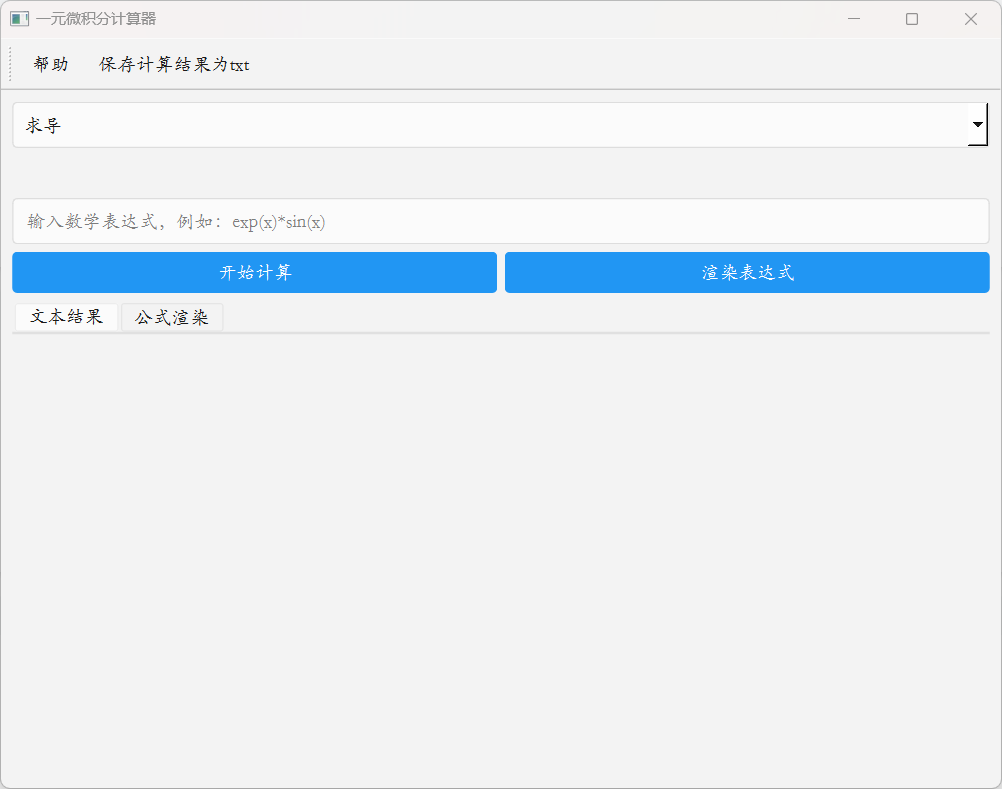
\includegraphics[width=1.0\linewidth]{主界面}
		\caption{主界面}
		\label{fig:mainwindow}
	\end{figure}
	\begin{figure}[H]
		\centering
		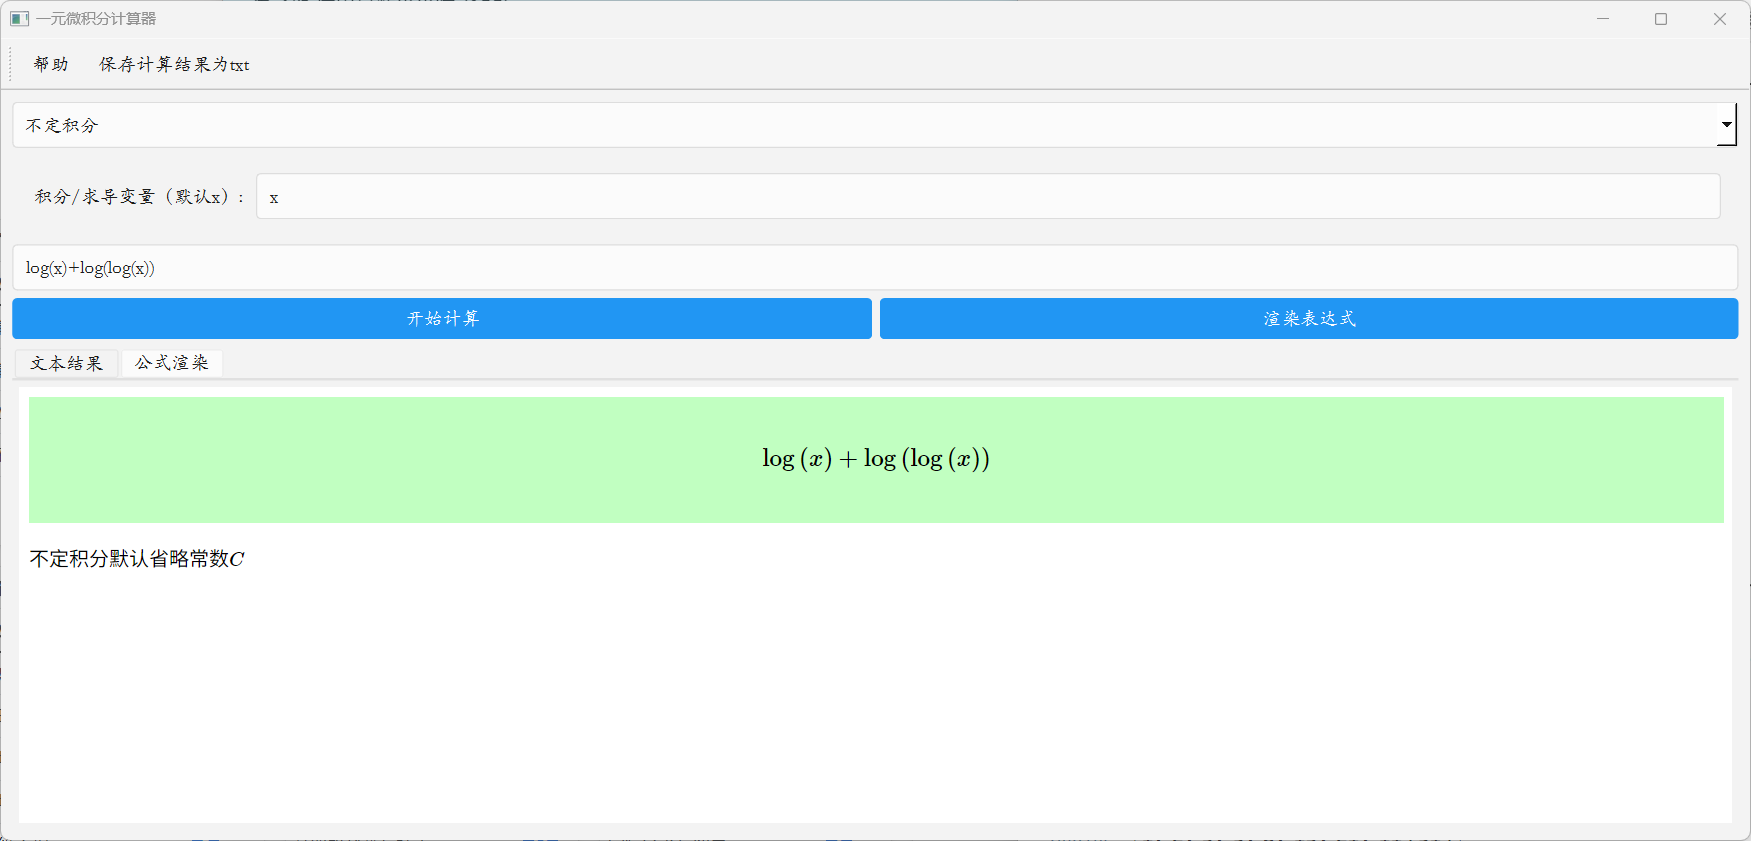
\includegraphics[width=1.0\linewidth]{渲染表达式}
		\caption{公式渲染}
		\label{fig:latex}
	\end{figure}
	\begin{figure}[H]
		\centering
		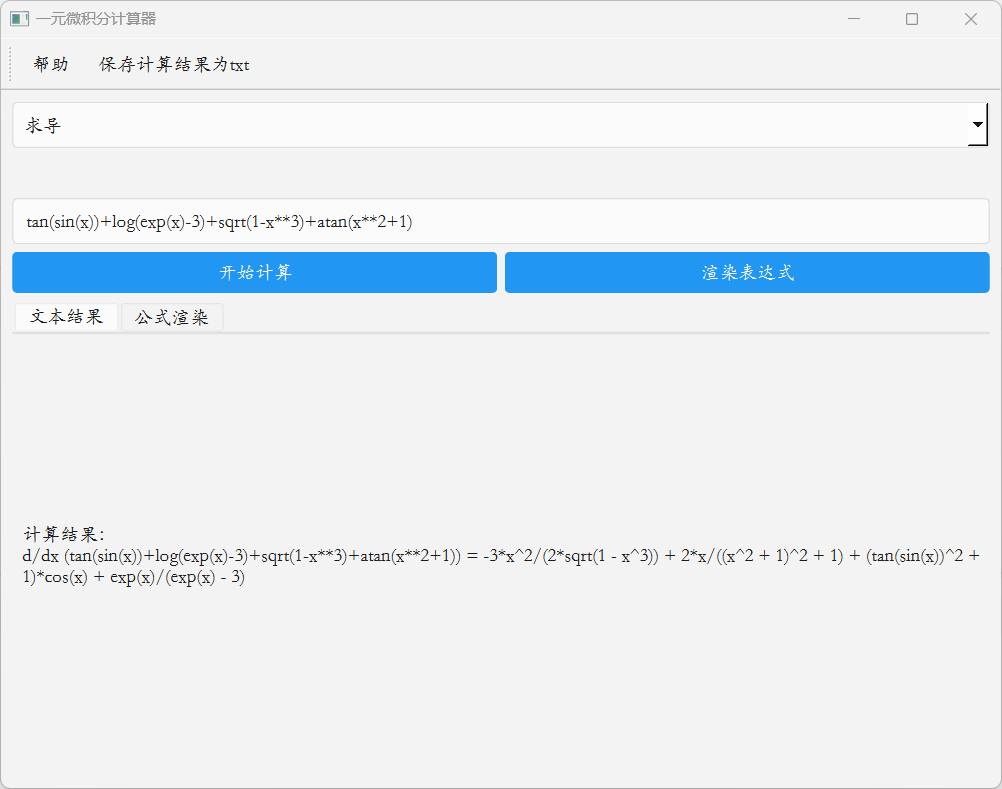
\includegraphics[width=1.0\linewidth]{求导计算_文字结果}
		\caption{求导计算:文字结果}
		\label{fig:dif_text}
	\end{figure}
	\begin{figure}[H]
		\centering
		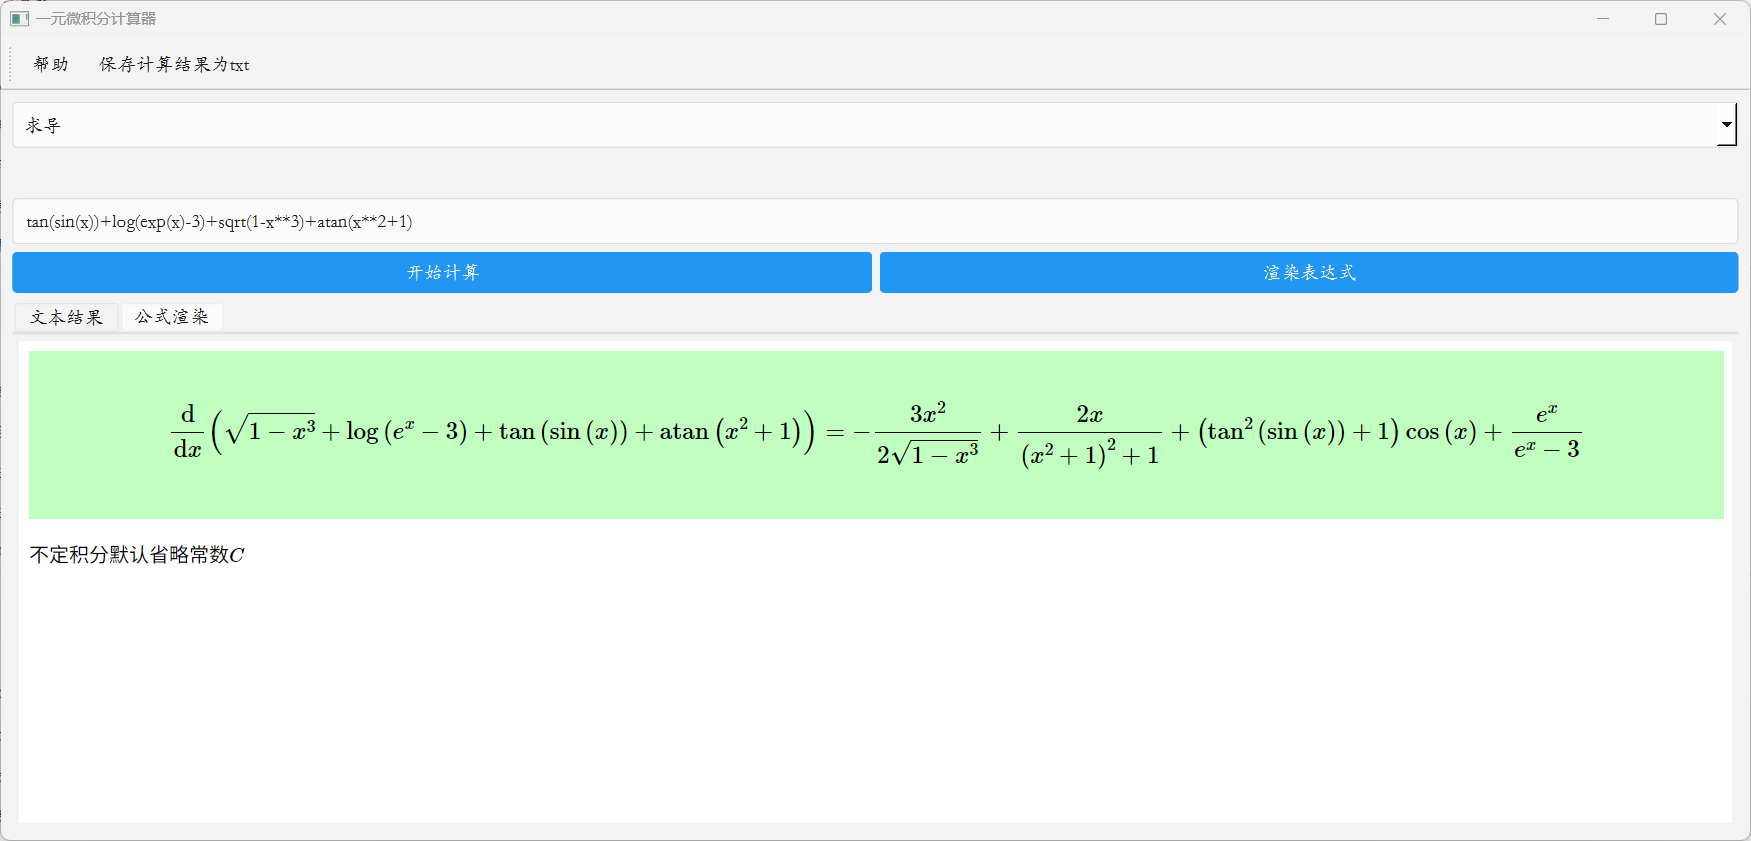
\includegraphics[width=1.0\linewidth]{求导计算_公式渲染}
		\caption{求导计算:公式渲染}
		\label{fig:dif_latex}
	\end{figure}
	\begin{figure}[H]
		\centering
		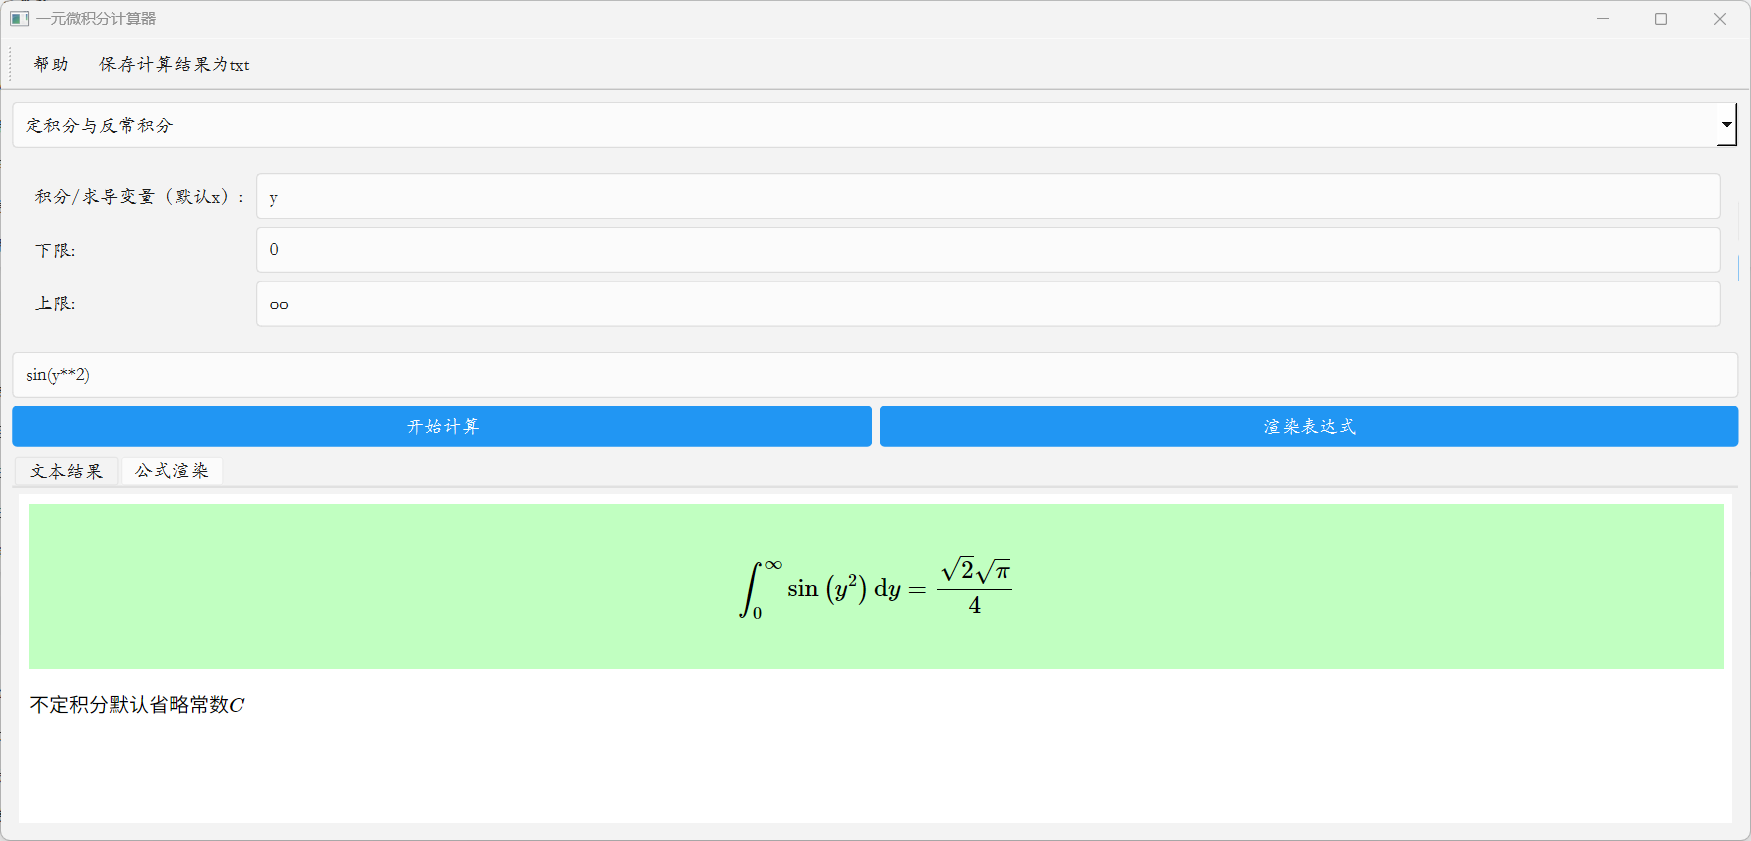
\includegraphics[width=1.0\linewidth]{定积分与反常积分计算_公式渲染}
		\caption{定积分与反常积分计算:公式渲染}
		\label{fig:deintegral}
	\end{figure}
	\begin{figure}[H]
		\centering
		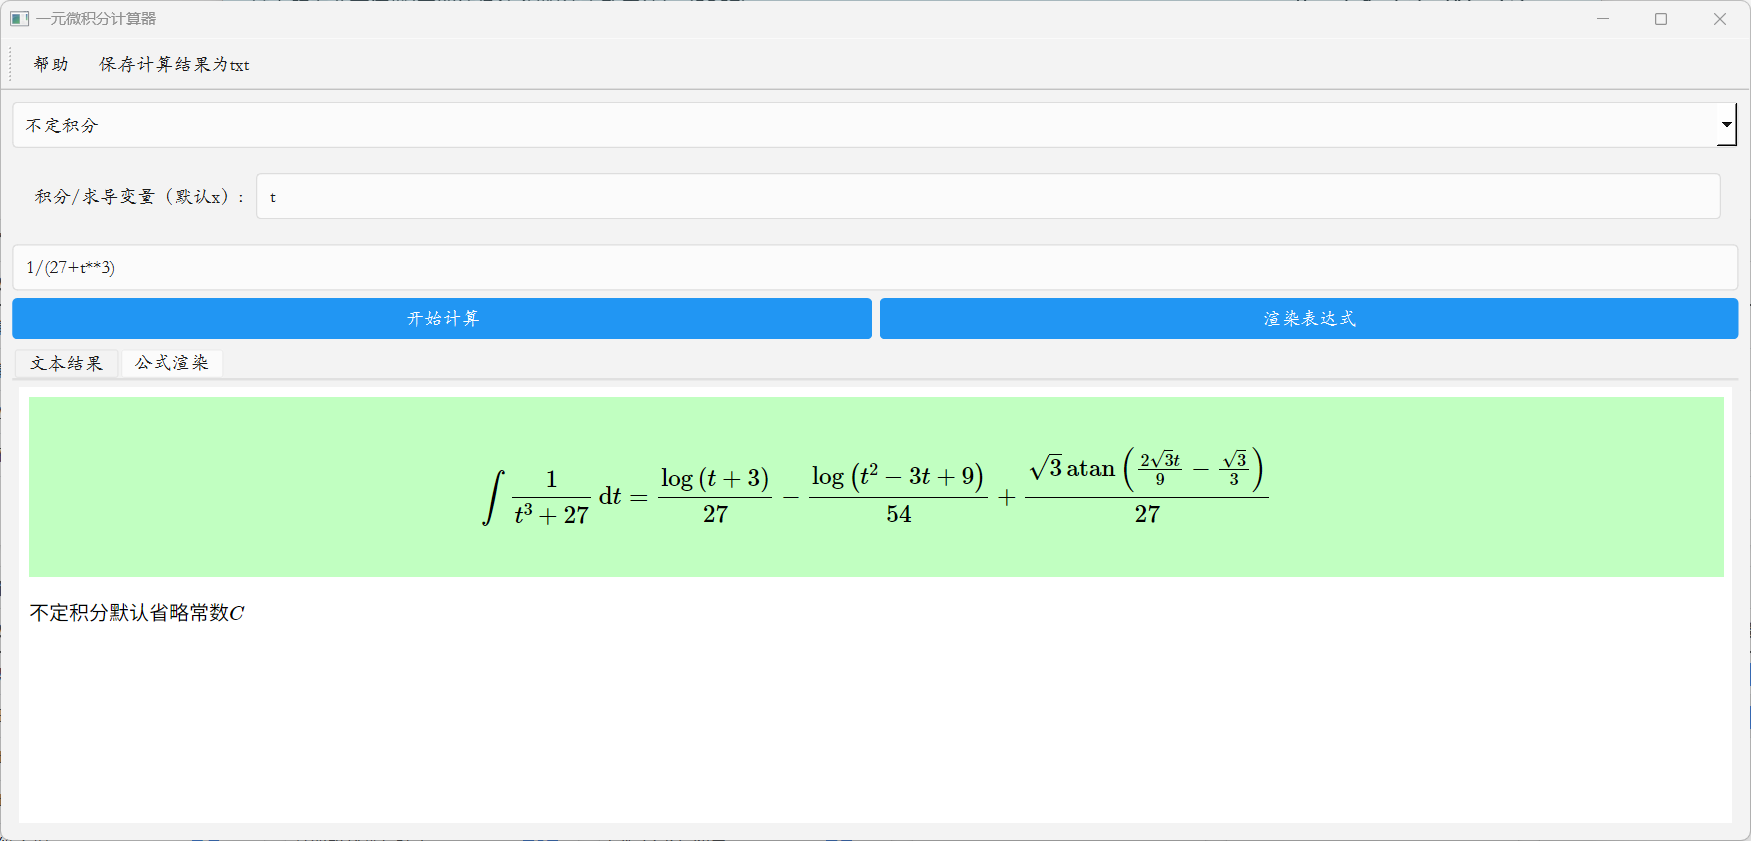
\includegraphics[width=1.0\linewidth]{不定积分计算_公式渲染}
		\caption{不定积分计算:公式渲染}
		\label{fig:integral}
	\end{figure}
	\begin{figure}[H]
		\centering
		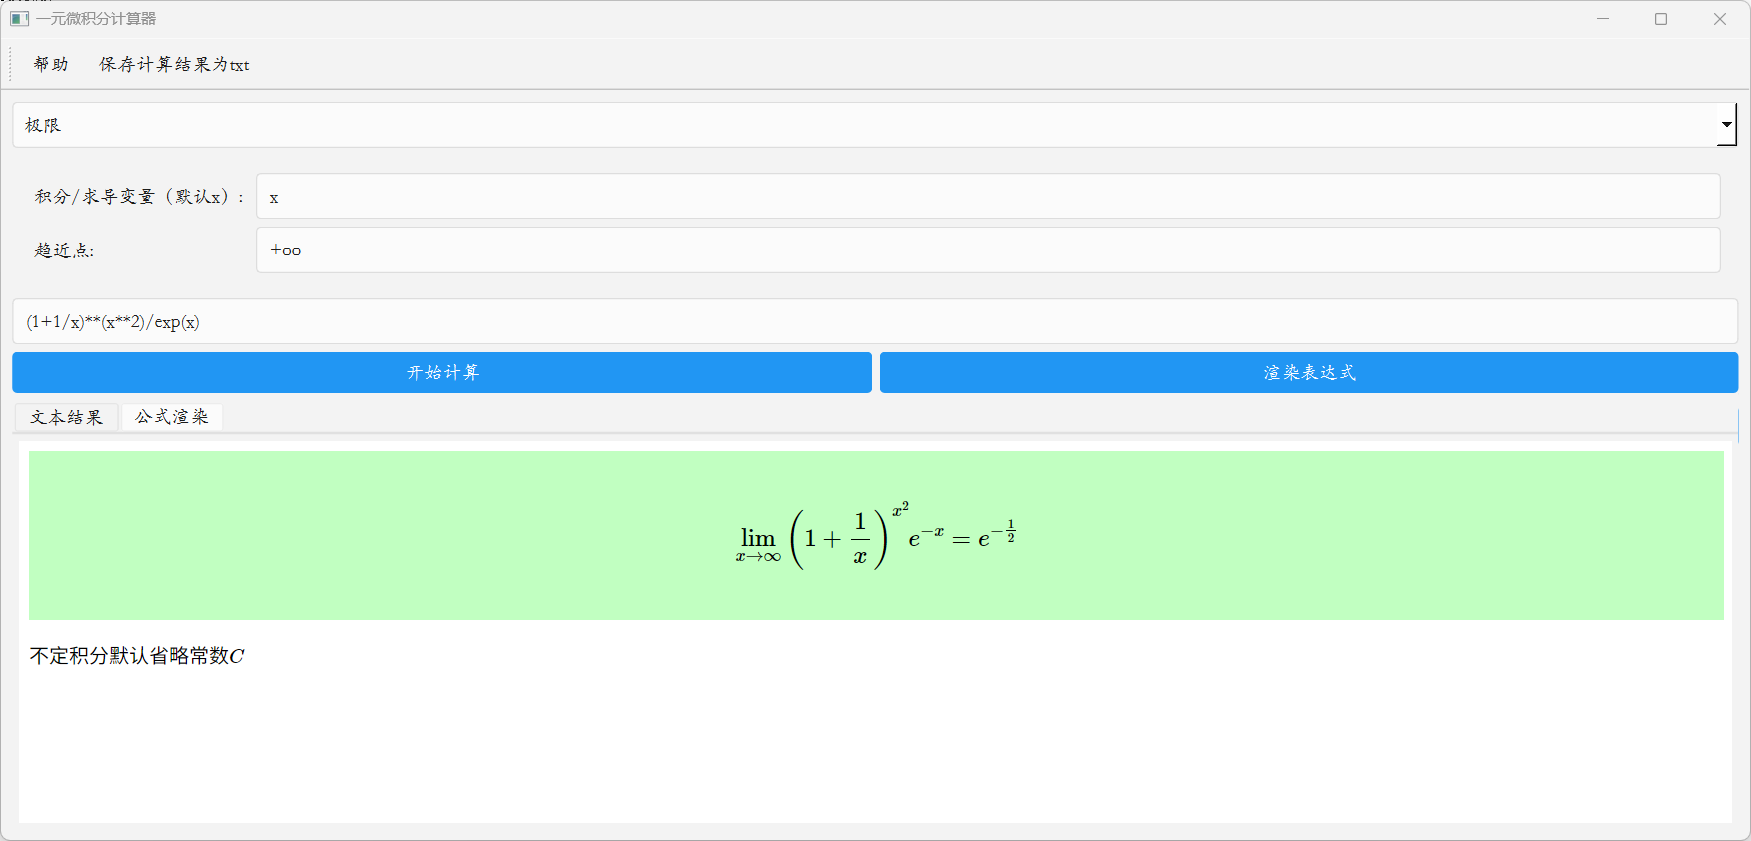
\includegraphics[width=1.0\linewidth]{极限计算_公式渲染}
		\caption{极限计算:公式渲染}
		\label{fig:limit}
	\end{figure}
	\begin{figure}[H]
		\centering
		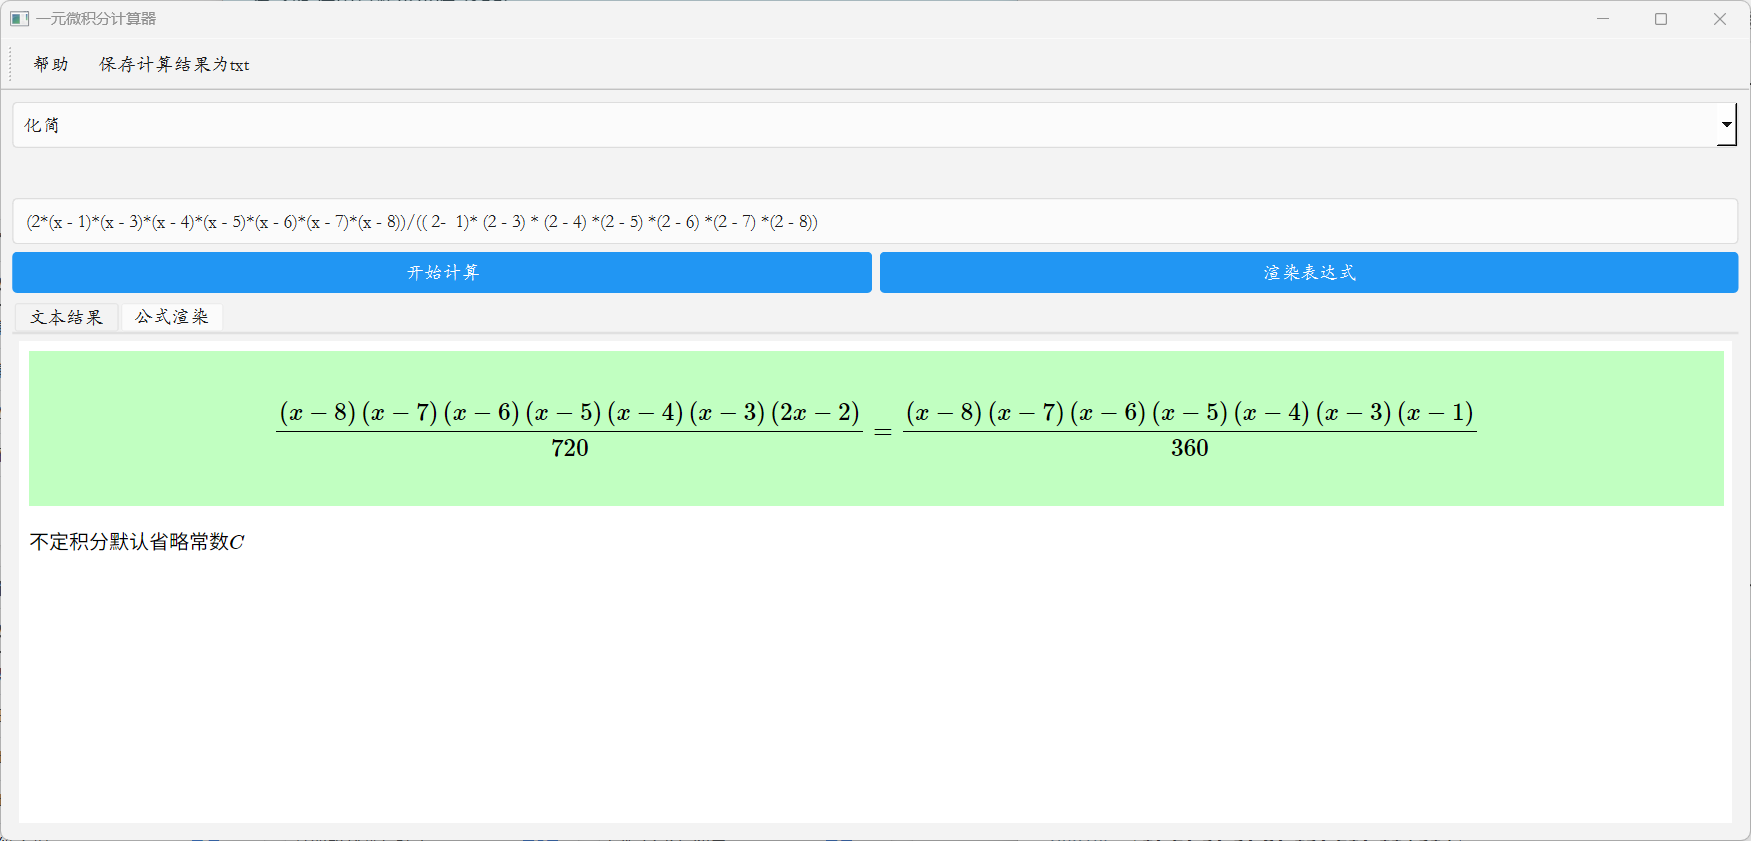
\includegraphics[width=1.0\linewidth]{化简_公式渲染}
		\caption{化简}
		\label{fig:simplify}
	\end{figure}
	\begin{figure}[H]
		\centering
		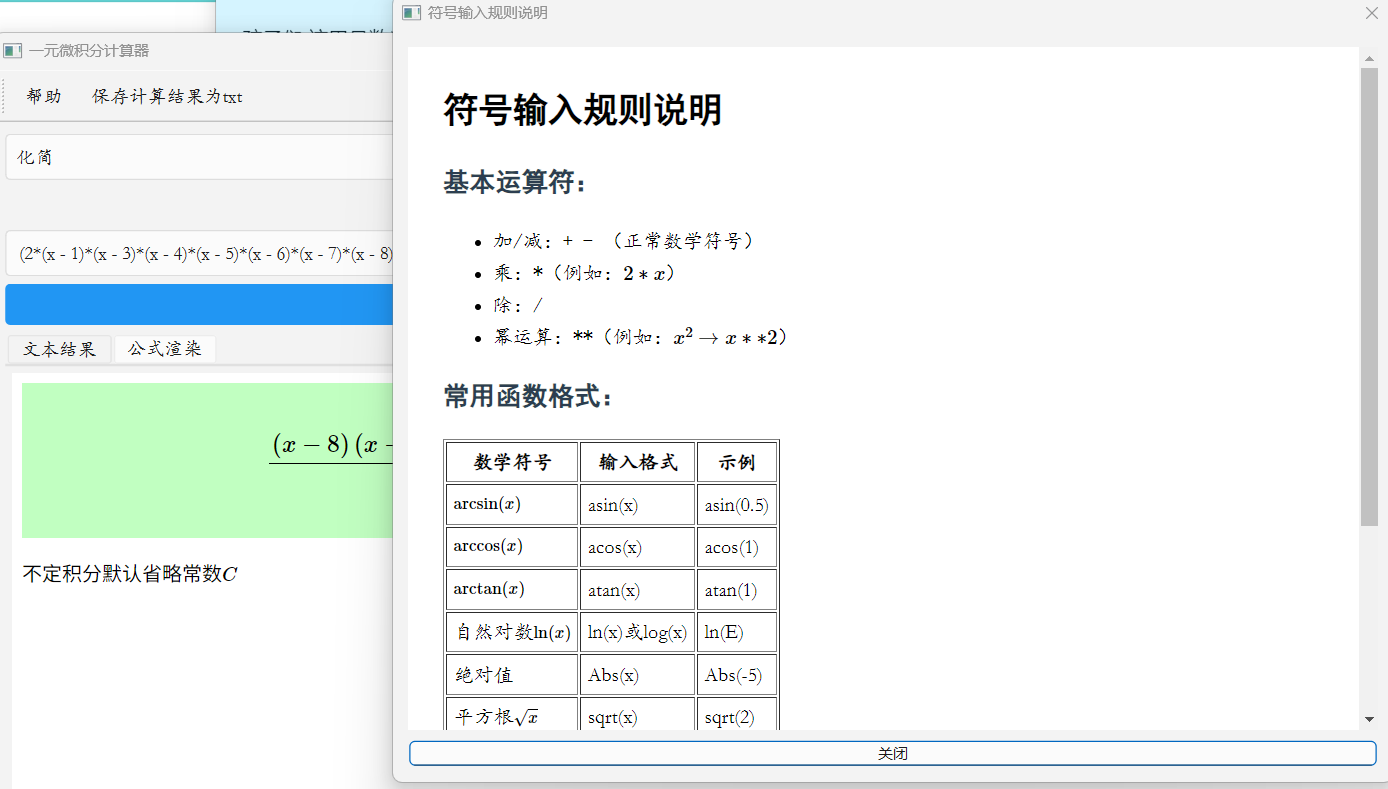
\includegraphics[width=1.0\linewidth]{帮助_界面}
		\caption{帮助界面}
		\label{fig:help}
	\end{figure}
	\begin{figure}[H]
		\centering
		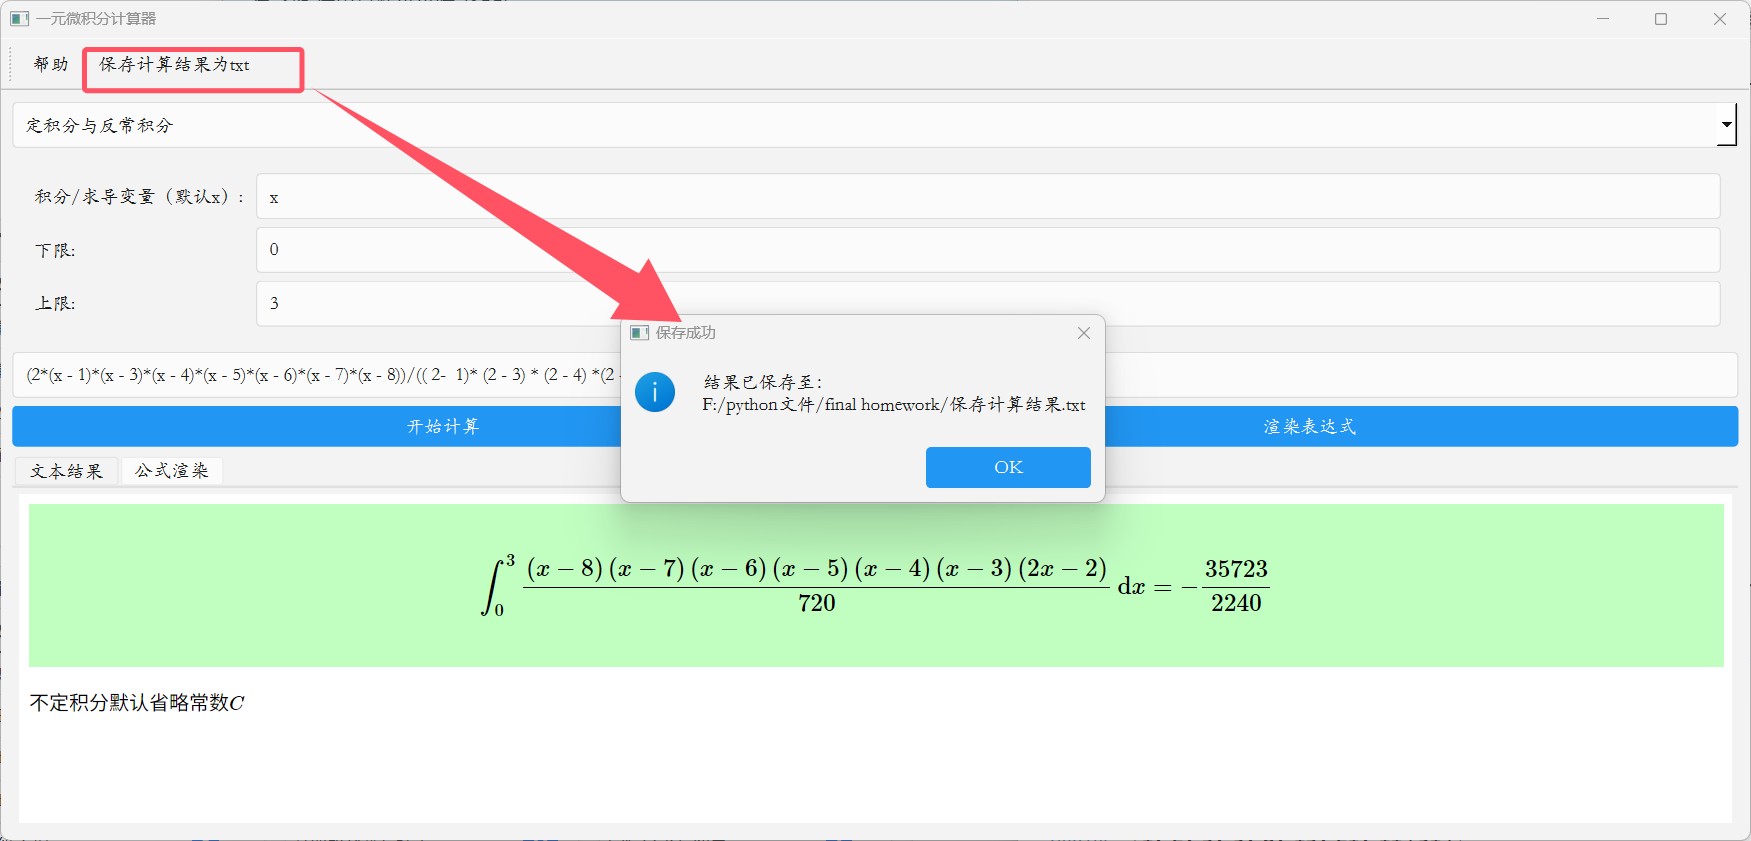
\includegraphics[width=0.7\linewidth]{保存计算结果}
		\caption{保存计算结果为txt文件}
		\label{fig:save}
	\end{figure}
	\section{总结与改进方向}
	\subsection{项目成果}
	\begin{itemize}
		\item 完整实现5类微积分运算(一元函数的极限、求导、不定积分、定积分与反常积分)与符号化简
		\item 开发响应式GUI界面
		\item 建立符号输入规范体系
	\end{itemize}
	
	\subsection{缺点与改进方向}
	\begin{enumerate}
		\item 有些较为复杂的积分计算无法算出,如\[\int_0^{\frac{\pi}2}\ln\sin x\,\mathrm dx=-\frac{\pi\ln 2}2\]无法计算,\[\int_0^1\frac{\arctan t}{t}\,\mathrm dt=\boldsymbol{G}\]也无法计算,这里的$\boldsymbol{G}$是Catalan常数. 
		\item 有些计算结果不是最简形式,如\[\int_0^{\pi/4}\tan x\,\mathrm dx=\frac{\ln 2}2,\]输出结果为$-\log\left(\frac{\sqrt2}2\right).$
		\item 不定积分计算没有加常数$C$.  关于一些化简计算不会原封不动地输出原始输入. 
		\item 有些函数的输入不太常用,如$\arctan(x)$也写成$\operatorname{atan}(x)$
		\item 所有自然对数的输出都是$\log x$而不是常用的$\ln x$.
		\item 仅支持$x,y,z,t$作为变量; 
		\item \textbf{功能扩展}:支持的功能还不够丰富,但是没时间制作了,还可以完善如下内容\begin{enumerate}
			\item 函数在某点的Taylor级数展开;
			\item 数值计算;
			\item 判断表达式的真假;
			\item 解方程,例如求解多项式的根和某些微分方程;
			\item 线性代数功能,例如线性方程组的求解,矩阵的加法、数乘、乘法、转置、逆,判断矩阵的秩,计算方阵的行列式和特征值等. 
		\end{enumerate}
		\item \textbf{性能优化}:引入计算缓存机制
		\item \textbf{可视化增强}:支持2D/3D图形绘制
	\end{enumerate}
	
\end{document}